\chapter{\IfLanguageName{dutch}{Proof-of-Concept}{Proof-of-Concept}}%
\label{ch:proof-of-concept}

% Tip: Begin elk hoofdstuk met een paragraaf inleiding die beschrijft hoe
% dit hoofdstuk past binnen het geheel van de bachelorproef. Geef in het
% bijzonder aan wat de link is met het vorige en volgende hoofdstuk.

% Pas na deze inleidende paragraaf komt de eerste sectiehoofding.

In dit hoofdstuk worden de verschillende fases van het Proof-of-Concept beschreven. Deze werd opgesteld op basis van de requirements-analyse (zie \ref{sec:requirements-analyse}). Het eerste deel van dit hoofdstuk gaat de opzetting in detail beschrijven. Deze begint met de implementatie van de React-website als grote basis, en verdiept zich vervolgens in de specifieke implementatie en conversie naar de React Native en Ionic applicaties. Het tweede deel bestaat uit de analyse van deze applicaties, waarbij de performantie en de verschillen worden onderzocht aan de hand van testscenario's. Deze resultaten worden nader verklaard en geïnterpreteerd in een volgende hoofdstuk.

%Voor de opzetting, werd er gekozen om te vertrekken vanuit een algemene React-website. Zowel React Native als Ionic maken gebruik van React, waardoor de algemene structuur van de applicatie al kon worden vastgesteld.

\section{Opzetten van Proof-of-Concept}
\label{sec:opzetten-proof-of-concept}

\subsection{Back-end}
\label{subsec:back-end}

Zoals eerder vermeld in de requirements-analyse, is de back-end ontwikkeld met behulp van Express v4.19.2. Deze bestaat uit één enkele API-endpoint die verantwoordelijk is voor het verwerken van HTTP-verzoeken naar specifieke video's die lokaal zijn opgeslagen. De code maakt gebruik van de fs-module van Node.js om toegang te krijgen tot deze lokale videobestanden. De bestanden zelf zijn van het bestandstype .mkv en variëren in zowel bestandgrootte en resolutie om een zo breed mogelijk spectrum van streaming te kunnen testen.

Wanneer de back-end een GET-request ontvangt op de url '/videos/:file', waarbij ':file' een voorgedefinieerde constante is die hoort bij een specifieke video, zal de padnaam voor de desbetreffende video worden opgezocht via een gedefinieerde mapping. Hierna wordt via de fs-module \verb|fs.statSync(filepath)| opgeroepen om bepaalde gegevens over het bestand op te halen. Dit is belangrijk om bijvoorbeeld de grootte van het bestand te kunnen bepalen die op zijn beurt weer nodig is om de video in pakketten te kunnen streamen. Indien er geen videobestand is gevonden, zal de back-end een 404-error terugsturen naar de client.

Hieropvolgend wordt er gecontroleerd of het verzoek een bereik van bytes bevat door de 'range' header van de inkomende request te inspecteren met \verb|req.headers.range|. In dit geval betekent dit dat de client een deel van het bestand wil gaan streamen in plaats van in zijn volledigheid te downloaden. Het start- en eindpunt van het bereik wordt geëxtraheerd uit deze ontvangen 'range' header via reguliere expressies. De volgende stap is het bepalen van de grootte van de chunk, of ook wel het deel van het bestand dat moet worden gestreamd. Dit wordt berekend aan de hand van verschillende variabelen, zoals de start- en eindpunten die weer gebruikmaken van de eerder genoemde 'range' header. Vervolgens wordt er een \verb|ReadStream|  aangemaakt voor dit specifieke gedeelte van het bestand met behulp van \verb|fs.createReadStream| \verb|(filePath, |\verb|{ start, end })|.

De laatste stappen bestaan uit het toekennen van de juiste HTTP-headers voor de response en deze een statuscode van '206 Partial Content' mee te geven. Dit wil zeggen dat de server slechts een deel van de data effectief doorstuurt naar de client. Zo bevatten de headers daarnaast ook informatie over het bereik van de bytes dat wordt verzonden en de grootte van de chunk. Deze worden vervolgens allemaal toegekend aan het response object met \verb|res.writeHead(206, head)|. Tot slot wordt de \verb|ReadStream| doorgegeven aan het response object met \verb|file.pipe(res)|. Dit zorgt ervoor dat de data van de chunk wordt doorgestuurd naar de client op een performante manier, in plaats van het volledige bestand in één keer te moeten inladen.

De volledige code van de back-end op basis van bovenstaande uitleg ziet er zo uit:

\begin{mdframed}[backgroundcolor=bg]
  \begin{minted}[breaklines]{jsx}
app.get('/videos/:file', (req, res) => {
    // Ophalen van de bestandsnaam met de file parameter
    // uit de URL
    const fileName = req.params.file;
    const filePath = videoFileMap[fileName];
    if (!filePath) {
      // Indien het bestand niet gevonden is, stuur een
      // 404-error terug
      return res.status(404).send('File not found');
    }

    // Ophalen van de bestandsinformatie
    const stat = fs.statSync(filePath);
    const fileSize = stat.size;
    const range = req.headers.range;

    if (range) {
      // Indien er een bereik van bytes is opgegeven, moet er
      // slechts een deel van het bestand worden teruggestuurd
      const parts = range.replace(/bytes=/, "").split("-");

      // Bepalen van het start- en eindpunt van het bereik
      const start = parseInt(parts[0], 10);
      const end = parts[1] ? parseInt(parts[1], 10) : fileSize - 1;

      // Bepalen van de grootte van de chunk
      const chunksize = (end - start) + 1;

      // Aanmaken van een ReadStream voor het specifieke deel
      // van het bestand
      const file = fs.createReadStream(filePath, { start, end });

      // Toekennen van de juiste HTTP-headers
      const head = {
        'Content-Range': `bytes ${start}-${end}/${fileSize}`,
        'Accept-Ranges': 'bytes',
        'Content-Length': chunksize,
        'Content-Type': 'video/mkv',
      };

      // Sturen van de response met statuscode 206 Partial
      // Content en de juiste headers
      res.writeHead(206, head);

      // Doorsturen van de data naar het response-object
      file.pipe(res);
    }
    else {
      // Indien er geen bereik van bytes is opgegeven,
      // stuur het volledige bestand
      const head = {
        'Content-Length': fileSize,
        'Content-Type': 'video/mkv',
      };

      // Statuscode 200 en de juiste headers toekennen
      res.writeHead(200, head);
      // Doorsturen van de data naar het response-object
      fs.createReadStream(filePath).pipe(res);
    }
});
  \end{minted}
\end{mdframed}


\subsection{React-website}
\label{subsec:react-website}

De volgende stap in het POC-proces, is het opzetten van een React-website. Deze website dient als basis voor zowel de Ionic-applicatie als de React Native-applicatie. Deze bestaat uit een zeer eenvoudige gebruikersinterface met een beperkt aantal functionaliteiten die werden bepaald in de eerder besproken requirements-analyse. De website bestaat dus uit een Header, een VideoPlayer-component en een aantal knoppen die elk een specifieke video vertegenwoordigen. De gebruiker kan op deze knoppen klikken om de bijhorende video af te spelen in de VideoPlayer-component. De website is daarnaast ontworpen met een beperkt responsief ontwerp in gedachten, zodat deze ondersteund is voor zowel de browser als voor de mobiele Ionic-versie.

In het bestand 'App.js' wordt de hoofdstructuur van de website gedefinieerd. Allereerst wordt er binnen deze App-component een state bijgehouden voor de 'videoId' (ook wel de voorgedefinieerde constante die hoort bij een specifieke video uit de back-end) met behulp van de 'useState'-hook en wordt deze geïnitialiseerd met \verb|null|. Deze state houdt bij welke video momenteel wordt afgespeeld in de VideoPlayer-component.

Vervolgens is er een \verb|playVideo|-functie gedefinieerd binnenin de App-component. Deze functie wordt aangeroepen wanneer een van de afspeelknoppen wordt aangeklikt. De \verb|e.preventDefault()| -functie wordt aangeroepen om het eventuele standaardgedrag dat ontstaat bij het klikken op een knop te voorkomen. Het zou bijvoorbeeld kunnen voorkomen dat de pagina opnieuw wordt geladen. Daarna wordt via de \verb|setVideoId|-functie de 'videoId'-state bijgewerkt naar de nieuwe waarde die overeenkomt met de gekozen video.

Als laatste retourneert deze component nog de JSX, of ook wel de daadwerkelijke interface van de website. Deze bestaat uit pure HTML in combinatie met de Header-, VideoPlayer- en de Button-componenten. Indien een button wordt aangeklikt, zal de \verb|playVideo|-functie aangeroepen worden en dus bijgevolg de 'videoId'-state worden bijgewerkt. Deze ID wordt op zijn beurt dan weer doorgegeven aan de VideoPlayer-component als parameter. Deze code van de App-component luidt als volgt:


\begin{mdframed}[backgroundcolor=bg]
  \begin{minted}[breaklines]{jsx}
function App() {
    // State voor de videoId
    const [videoId, setVideoId] = useState(null);

    // Functie om een video af te spelen bij het 
    // klikken op een knop
    function playVideo(e, videoId) {
      e.preventDefault();
      setVideoId(videoId);
    };

    // Retourneren van de JSX
    return (
      <div className="App">
        <Header/>
        <div className='content'>
          <div className='player'>
            {videoId && <VideoPlayer videoId={videoId}></VideoPlayer>} <br />
          </div>
          <div className='vidSelect'>
            <button onClick={(e) => playVideo(e, 'got')}>
              Play GOT trailer
            </button>
            <button onClick={(e) => playVideo(e, 'tlou')}>
              Play TLOU trailer
            </button>
            <button onClick={(e) => playVideo(e, 'dune')}>
              Play DUNE 2 4k trailer
            </button>
          </div>
        </div>
      </div>
    );
}
  \end{minted}
\end{mdframed}


\begin{figure}
  \centering
  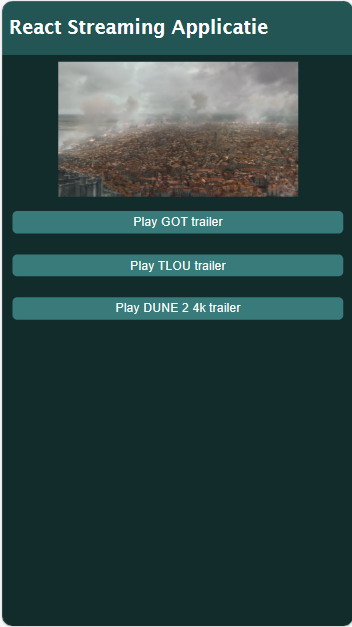
\includegraphics[width=0.7\linewidth]{img/ReactWebsiteIphone}
  \caption{React-website op een iPhone SE vanuit de browser.}
  \label{fig:React-website op een iPhone SE vanuit de browser}
\end{figure}

De volgende en ook wel belangrijkste component in dit POC, is de VideoPlayer-component. Deze is verantwoordelijk voor het effectief afspelen van de geselecteerde video. Deze ontvangt ten eerste een 'videoId' als parameter. Wanneer de 'videoId' zou veranderen in de App-component, zoals bij het aanklikken van een van bovenstaande knoppen, zal deze component volledig opnieuw renderen.

De VideoPlayer maakt daarnaast eerst en vooral gebruik van de 'useRef'-hook om een referentie te verkrijgen naar het <video>-element. Dit is nodig om toegang te verkrijgen tot de video zelf en om bepaalde eigenschappen te kunnen wijzigen. Dit wordt gedaan in de 'useEffect'-hook van de code. Het nut van deze hook is dat deze wordt aangeroepen na de eerste render van de component en na elke volgende update. Dit laat toe om bepaalde side-effects op te lossen. De rol van deze hook heeft vooral te maken met het re-renderen van de VideoPlayer indien de 'videoId' verandert. In dit geval zal de video gepauzeerd worden, de huidige source naar de video verwijderd worden en de video met de nieuwe source correct laden en afspelen. Zonder deze useEffect-hook zou indien een nieuwe video geselecteerd is, deze niet kunnen ingeladen worden en nog steeds een referentie hebben naar de oude source.

Tot slot retourneert deze component een <video>-element waarin de video wordt afgespeeld. De grootte van het video-element wordt dynamisch ingesteld op basis van de 'vidWidth' en 'vidHeight'-states uit de component. De source van de video wordt dynamisch toegekend aan de hand van een url naar de back-end API endpoint met de 'videoId' als parameter.

De code van de VideoPlayer ziet er als volgt uit. Om de leesbaarheid te verhogen tot enkel de belangrijkste aspecten uit de code, zijn enkele lijntjes code weggelaten die betrekking hebben tot de grootte van het venster van de video zelf. Deze hebben echter geen invloed op de prestaties van de website en/of applicatie zelf en behoren ook niet tot de scope van dit onderzoek. Let hierbij op dat de url naar de back-end deels is vervangen door de letter 'X' om privacyredenen. Dit kan vervangen worden door 'localhost', maar bleek de enige oplossing voor de Ionic-applicatie om lokaal de back-end te bereiken.

\begin{mdframed}[backgroundcolor=bg]
  \begin{minted}[breaklines]{jsx}
const VideoPlayer = ({videoId}) => {
    // Referentie naar het video-element
    const videoRef = useRef(null);

    // UseEffect om de video te laden en af te spelen
    // wanneer de videoId verandert (enkel bij de eerste render)
    useEffect(() => {
      if (videoRef.current) {
        videoRef.current.pause();
        videoRef.current.removeAttribute('src');
        videoRef.current.load();
      }
    });

    // Retourneren van de JSX met het video-element
    return (
      <video ref={videoRef} width={vidWidth} height={vidHeight} controls>
        <source src={`http://192.168.X.XXX:3000/videos/${videoId}`}
          type="video/mkv"></source>
        Your browser does not support the video tag.
      </video>
    );
}
  \end{minted}
\end{mdframed}


\subsection{Ionic applicatie}
\label{sec:ionic-applicatie}

Nu de React-website is opgezet, kan er overgegaan worden tot het ontwikkelen en/of omzetten naar de mobiele applicaties. Uit Hoofdstuk \ref{sec:ionic} bleek dat er eigenlijk geen verdere aanpassingen hoeven te gebeuren aan de bestaande React-website om deze te kunnen omzetten naar een Ionic-applicatie. Ter verduidelijking werd er voor deze Ionic-applicatie gebruik gemaakt van het React-framework, alhoewel er hiervoor ook de keuze is om een andere, door Ionic ondersteund framework, te gebruiken. Dit heeft als troef dat de originele website-codebase letterlijk kan worden hergebruikt voor de mobiele applicatie.

Deze conversie gebeurt aan de hand van de Capacitor-plugin v6.0.0. De Ionic-applicatie zelf is dan weer gebouwd met versie 7.2.0 van Ionic. De combinatie van deze twee plugins maakt het mogelijk om de React-website te converteren naar een native-applicatie voor Android. Dit wordt bereikt door het aanmaken van twee bestanden: \verb|ionic.config.json| en \verb|capacitor.config.json|. Dit eerste bestand bevat de instellingen voor de Ionic-applicatie, zoals de naam en het feit dat deze applicatie steunt op React. Dit ziet er als volgt uit:

\begin{mdframed}[backgroundcolor=bg]
  \begin{minted}[breaklines]{json}
{
  "name": "IonicStreaming",
  "integrations": {
    "capacitor": {}
  },
  "type": "react"
}
  \end{minted}
\end{mdframed}

Het tweede bestand bevat dan weer configuraties voor de Capacitor-plugin. De inhoud hiervan ziet er zo uit:

\begin{mdframed}[backgroundcolor=bg]
  \begin{minted}[breaklines]{json}
{
  "appId": "io.ionic.IonicStreaming",
  "appName": "IonicStreaming",
  "bundledWebRuntime": false,
  "npmClient": "npm",
  "webDir": "build",
  "cordova": {}
}
  \end{minted}
\end{mdframed}

Na het aanmaken van deze bestanden is het nodig om de huidige website eerst te builden. Dit komt omdat Capacitor geen ingebouwde build-tool heeft en gebruik maakt van de bestaande build van de React-website. Door het commando \verb|npm run build| uit te voeren, worden de nodige bestanden gegenereerd in de 'build'-map in de root folder van het project. Er rest nog een laatste stap en dat is het effectief converteren naar een Android-applicatie. Het commando \verb|ionic capacitor| \verb|add android| zorgt hiervoor.

Nadat deze applicatie is geconverteerd, hebben we onze definitieve Ionic-applicatie. Dit zonder enig lijntje van de originele codebase aan te passen. De applicatie kan nu worden gebuild via Gradle en geïnstalleerd op een Android-toestel. Er is echter nog een klein probleem bij deze build en dit heeft allemaal te maken met de lokaal draaiende back-end. Omdat deze via de localhost bereikbaar is, moet het commando \verb|ionic cap run android| \verb|-l --external| worden uitgevoerd. Dit is enkel en alleen nodig in dit specifieke geval: indien de API-endpoint bereikbaar is via een externe HTTPS-verbinding, is dit niet nodig. Wat dit commando doet is de vorige stappen zelf opnieuw uitvoeren, maar de applicatie bovendien ook lokaal draaien op localhost. Dit kan best vergeleken worden met de Ionic-applicatie te draaien op een bepaalde poort, zoals de originele React-website zou doen. Door deze tussenstap te nemen, kan de app opgestart worden met Android Studio en toch de back-end via de lokale pc bereiken.

Een screenshot van de applicatie staat op de volgende pagina.

Door deze bovenstaande stappen te volgen was het dus mogelijk om zonder enige aanpassingen, de React-website te deployen als een native Android-applicatie. Dit toont aan dat de combinatie van React, Ionic en Capacitor een krachtige toolset is om webapplicaties om te zetten naar mobiele applicaties. Wat natuurlijk weer een voordeel is voor ontwikkelaars om niet een volledig nieuwe applicatie te moeten herimplementeren.

\subsection{React Native applicatie}
\label{sec:react-native-applicatie}

Het laatste deel van de opzetting voor de testscenario's is de React Native-conversie. In tegenstelling tot een Ionic-applicatie, steunt deze niet op de typische webtechnologie van HTML, maar maakt gebruikt van eigen custom componenten. Dit wil betekenen dat de React-website niet zomaar kan worden omgezet naar een React Native-applicatie zoals bij Ionic. Desondanks is deze omzetting wel mogelijk omdat React Native voor de meeste HTML-elementen een equivalent heeft. Dit laat toe om de meeste code toch op een relatief eenvoudige manier te kunnen hergebruiken, mits enkele aanpassingen die hier worden besproken.

\begin{figure}
  \centering
  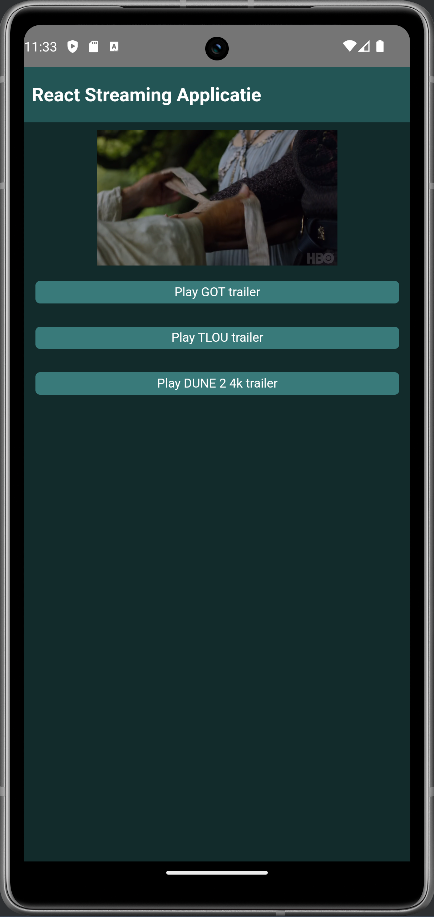
\includegraphics[width=0.7\linewidth]{img/ReactIonicPhone}
  \caption{Ionic-applicatie op een Google Pixel 7a}
  \label{fig:Ionic-applicatie op een Google Pixel 7a}
\end{figure}

\begin{mdframed}[backgroundcolor=bg]
  \begin{minted}[breaklines]{jsx}
const App = () => {
    // State voor de videoId
    const [videoId, setVideoId] = useState(null);

    // Functie om een video af te spelen bij het klikken
    // op een knop
    function playVideo(e, videoId) {
      e.preventDefault();
      setVideoId(videoId);
    };

    // Retourneren van de JSX met de Header-, VideoPlayer-
    // en Button-componenten
    return (
      <View style={styles.app}>
        <Header />
        <View style={styles.content}>
            <VideoPlayer videoId={videoId}></VideoPlayer>
            <View style={styles.vidSelect}>
              <Button
                onPress={(e) => playVideo(e, 'got')}
                title='Play GOT trailer'
                color={'rgb(57, 122, 122)'}>
              </Button>
              <Button
                onPress={(e) => playVideo(e, 'tlou')}
                title='Play TLOU trailer'
                color={'rgb(57, 122, 122)'}>
              </Button>
              <Button
                onPress={(e) => playVideo(e, 'dune')}
                title='Play DUNE 2 4k trailer'
                color={'rgb(57, 122, 122)'}>
              </Button>
          </View>
        </View>
      </View>
    );
};
  \end{minted}
\end{mdframed}

Bovenstaande code toont de App-component van de React Native-applicatie. Deze is zeer gelijkaardig aan de App-component van de originele React-website. Het grootste verschil is dat de HTML-elementen vervangen zijn door React Native- componenten. Zo wordt de <div>-tag vervangen door de <View>-tag en de HTML-buttons door de <Button>-component. De styling werd ook identiek overgezet op basis van de React-website, maar heeft eigenlijk geen invloed op de werking van de applicatie zelf. Als er vervolgens gekeken wordt naar de VideoPlayer-component, is deze ook gelijkaardig opgebouwd als de React-website. Maar voor deze component bleek er toch één groot probleem: React Native biedt geen standaard video-component aan. Dit betekent dus dat er moet gesteund worden op een externe package. In dit geval werd er gekozen voor de 'react-native-video'-package. Deze light-weight package biedt een video-component aan die zeer gelijkaardig is aan de <video>-tag in HTML.

Er wordt daarnaast opnieuw gebruikt gemaakt van de 'useRef'-hook om een referentie te verkrijgen naar het video-element. De useEffect-hook bij Ionic wordt echter niet gebruikt aangezien de React Native-video-component zelf al een ingebouwde manier heeft om de video te pauzeren en te hervatten, en de source van de video automatisch laat wijzigen wanneer de 'videoId' verandert. Deze useEffect-hook is dus overbodig in dit geval.

Voor de connectie met localhost is er geen extra configuratie nodig zoals bij de Ionic-applicatie. Slechts de url zoals in de onderstaande code bleek voldoende voor de connectie:

\begin{figure}
  \centering
  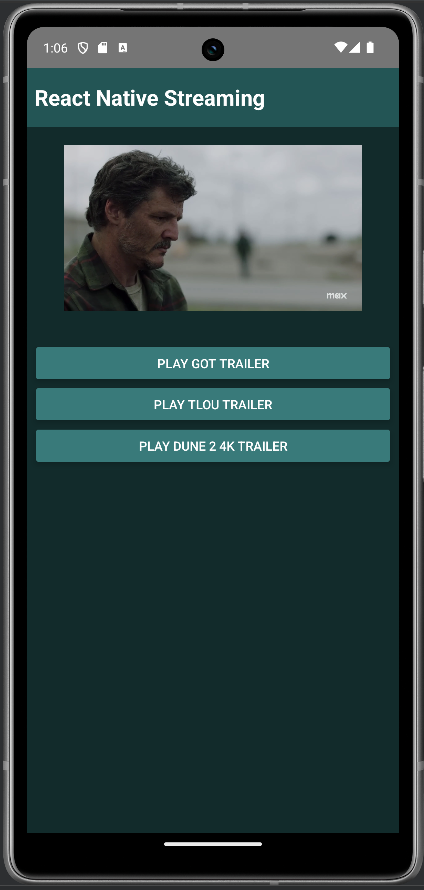
\includegraphics[width=0.7\linewidth]{img/ReactNativePhone}
  \caption{React Native-applicatie op een Google Pixel 7a}
  \label{fig:React Native-applicatie op een Google Pixel 7a}
\end{figure}

\begin{mdframed}[backgroundcolor=bg]
  \begin{minted}[breaklines]{jsx}
const VideoPlayer = ({videoId}) => {
    // Referentie naar het video-element
    const videoRef = useRef(null);

    // Retourneren van de JSX met de video-component
    // van de react-native-video package
    return (
      <View style={styles.videoView}>
        <Video 
          source={{uri: `http://10.0.2.2:3000/videos/${videoId}`}} 
          ref={(ref) => {
            videoRef.current = ref;
          }}         
          style={styles.backgroundVideo}
        />
      </View>
    );
}
  \end{minted}
\end{mdframed}

Nu de code is geschreven is het enkel nog een kwestie van de applicatie te builden en te deployen naar een Android-toestel. Hiervoor werd er in de package.json volgende script toegevoegd:

\begin{mdframed}[backgroundcolor=bg]
  \begin{minted}[breaklines]{json}
"build": "react-native bundle --platform android --dev false --entry-file index.js --bundle-output android/app/src/main/assets/index android.bundle --assets-dest android/app/src/main/res"
  \end{minted}
\end{mdframed}

%++ metro v0.80.8

Dit script zorgt ervoor dat de code wordt gebundeld en dat de nodige bestanden worden gegenereerd in de 'android/app/src/main/assets'-map van de root-folder. Vervolgens kan deze build worden geopend in Android Studio en kan de applicatie via Gradle worden gebuild en geïnstalleerd op een Android-toestel. De afbeelding op de vorige pagina toont de React Native-applicatie op een Google Pixel 7a. Enkele verschillen zijn misschien merkbaar in de styling tussen de verschillende versies, maar dit heeft opnieuw geen invloed op de performantie van de applicatie en eerder te maken met de beperkte styling die React Native aan zijn componenten geeft. Bovendien werd de styling zo goed als helemaal overgenomen van de originele React-website (en dus ook Ionic-applicatie), dus deze kleine verschillen zijn als het ware verwaarloosbaar.

\section{Testscenario's}
\label{sec:testscenario}

Gezien de ontwikkeling van zowel de Ionic- als de React Native-applicaties nu voltooid is, kan er overgegaan worden naar de testfase van deze Proof-of-Concept. In deze fase zal er onder andere gekeken worden naar de algemene opstarttijden, gebruikerservaring bij de interactie met de applicatie, alsook metingen worden gedaan met betrekking tot het CPU- en geheugenverbruik.


\subsection{Cold startup-tijd}
\label{subsec:cold-startup-tijd}

De term cold startup-tijd verwijst naar de tijd die nodig is voor een applicatie om op te starten vanaf het begin. Dit in een situatie waarbij de applicatie nog niet is geopend (zoals bij het opstarten van het toestel) of na het volledig afsluiten van de app. Deze meting werd uitgevoerd door de applicatie eerst telkens volledig af te sluiten door een 'force stop' uit te voeren op de emulator en vervolgens de applicatie opnieuw te openen. Aan de hand van de logs en de Profiler van Android Studio kon de tijd gemeten worden vanaf het aanklikken van het icoon, tot wanneer de componenten volledig zijn ingeladen op het scherm. Er valt hierbij op te merken dat de videocomponent nog niet wordt ingeladen vanwege het feit dat er geen video is geselecteerd. Dit wordt in een latere fase onderzocht.

De resultaten na twintig metingen zijn te zien in tabel \ref{tab:cold_startup}.

\begin{table}[htbp]
  \centering
  \begin{tabular}{|c|c|c|}
    \hline
    \textbf{Testscenario} & \textbf{Ionic} & \textbf{React Native} \\
    \hline
    1 & 2s 961ms & 6s 539ms \\
    \hline
    2 & 3s 114ms & 6s 876ms \\
    \hline
    3 & 3s 191ms & 6s 967ms \\
    \hline
    4 & 2s 987ms & 6s 477ms \\
    \hline
    5 & 3s 73ms & 6s 826ms \\
    \hline
    6 & 3s 118ms & 6s 895ms \\
    \hline
    7 & 2s 953ms & 6s 488ms \\
    \hline
    8 & 3s 2ms & 6s 611ms \\
    \hline
    9 & 3s 112ms & 6s 524ms \\
    \hline
    10 & 3s 148ms & 6s 450ms \\
    \hline
    11 & 3s 13ms & 6s 868ms \\
    \hline
    12 & 3s 205ms & 6s 813ms \\
    \hline
    13 & 2s 914ms & 6s 742ms \\
    \hline
    14 & 2s 902ms & 6s 499ms \\
    \hline
    15 & 3s 55ms & 6s 981ms \\
    \hline
    16 & 3s 70ms & 6s 827ms \\
    \hline
    17 & 2s 845ms & 6s 879ms \\
    \hline
    18 & 3s 113ms & 6s 624ms \\
    \hline
    19 & 2s 947ms & 6s 760ms \\
    \hline
    20 & 3s 6ms & 6s 855ms \\
    \hline
    \textbf{Gemiddelde} & \textbf{3s 36ms} & \textbf{6s 725ms} \\
    \hline
  \end{tabular}
  \caption{Cold startup tijd voor Ionic en React Native applicaties}
  \label{tab:cold_startup}
\end{table}

\begin{figure}
  \centering
  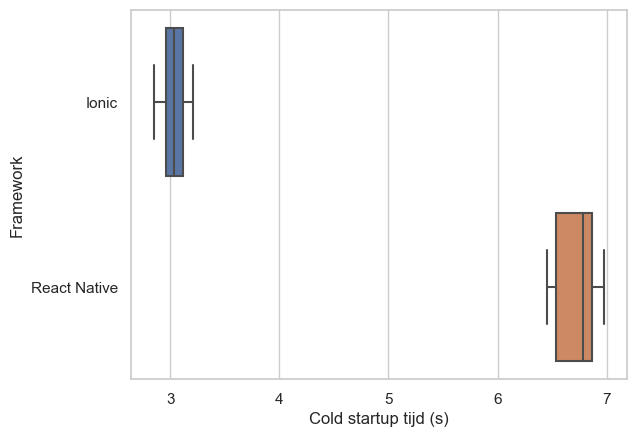
\includegraphics[width=0.7\linewidth]{img/boxplotCold}
  \caption{Boxplot van de cold startup-tijd voor Ionic en React Native applicaties}
  \label{fig:Boxplot van de cold startup-tijd voor Ionic en React Native applicaties}
\end{figure}

Deze resultaten werden vervolgens in een boxplot weergegeven om een beter beeld te verkrijgen van de spreiding van de data. Dit wordt weergegeven in Figuur \ref{fig:Boxplot van de cold startup-tijd voor Ionic en React Native applicaties}. Vervolgens werd er een t-test uitgevoerd om aan te tonen of er een significant verschil is tussen de gemiddelden van de cold startup-tijden bij Ionic en React Native. Als nulhypothese werd er vastgelegd dat er geen significant verschil is tussen de gemiddelden. De alternatieve hypothese, op basis van de boxplot en de tabel, was dat de resultaten voor Ionic lager zouden zijn dan die van React Native. De analyse werd uitgevoerd met een vastgesteld significantieniveau van \(0.05\). Uit deze test bleek dat de p-waarde \(1.312^{-36}\) bedroeg. Dit is aanzienlijk lager dat het significantieniveau en betekent dat de nulhypothese kan worden verworpen. Dit wijst er bovendien op dat de cold startup-tijden afhankelijk zijn van het type framework en dat Ionic inderdaad over snellere cold startup-tijden beschikt dan React Native. Dit kan een belangrijke factor zijn voor de gebruikerservaring van een applicatie. Een verdere verklaring en interpretatie van deze resultaten wordt, zoals eerder vermeld, gegeven in het volgende hoofdstuk.


\subsection{Warm startup-tijd}
\label{subsec:warm-startup-tijd}

Warm startup-tijd verwijst naar de tijd die nodig is voor een applicatie om opnieuw te starten nadat deze al een keer is gestart geweest en enige tijd inactief is. Dit is te vergelijken met een gebruiker die de applicatie opnieuw opent nadat deze al een keer is geopend en vervolgens is geminimaliseerd, om bijvoorbeeld te surfen op het internet. Dit omvat dus het opnieuw inladen van de applicatie, waarbij de resources voor een deel of volledig nog in het geheugen zijn opgeslagen. Deze meting werd uitgevoerd door de applicatie te openen, te minimaliseren, Google Chrome te openen en weer te minimaliseren, en vervolgens de Ionic- of React Native-app weer te openen. De tijd werd gemeten vanaf het aanklikken van het icoon tot wanneer de componenten volledig zijn ingeladen op het scherm op basis van de logs en de Profiler van Android Studio.

\begin{table}[htbp]
  \centering
  \begin{tabular}{|c|c|c|}
  \hline
  \textbf{Testscenario} & \textbf{Ionic} & \textbf{React Native} \\
  \hline
  1 & 239ms & 239ms \\
  \hline
  2 & 328ms & 237ms \\
  \hline
  3 & 301ms & 195ms \\
  \hline
  4 & 283ms & 232ms \\
  \hline
  5 & 241ms & 217ms \\
  \hline
  6 & 319ms & 200ms \\
  \hline
  7 & 281ms & 231ms \\
  \hline
  8 & 252ms & 204ms \\
  \hline
  9 & 302ms & 218ms \\
  \hline
  10 & 275ms & 245ms \\
  \hline
  11 & 236ms & 209ms \\
  \hline
  12 & 241ms & 233ms \\
  \hline
  13 & 291ms & 241ms \\
  \hline
  14 & 212ms & 226ms \\
  \hline
  15 & 333ms & 191ms \\
  \hline
  16 & 276ms & 221ms \\
  \hline
  17 & 273ms & 231ms \\
  \hline
  18 & 299ms & 208ms \\
  \hline
  19 & 269ms & 221ms \\
  \hline
  20 & 305ms & 213ms \\
  \hline
  \textbf{Gemiddelde} & \textbf{278ms} & \textbf{221ms} \\
  \hline
  \end{tabular}
  \caption{Warm startup-tijd voor Ionic en React Native applicaties}
  \label{tab:warm_startup}
\end{table}

\begin{figure}
  \centering
  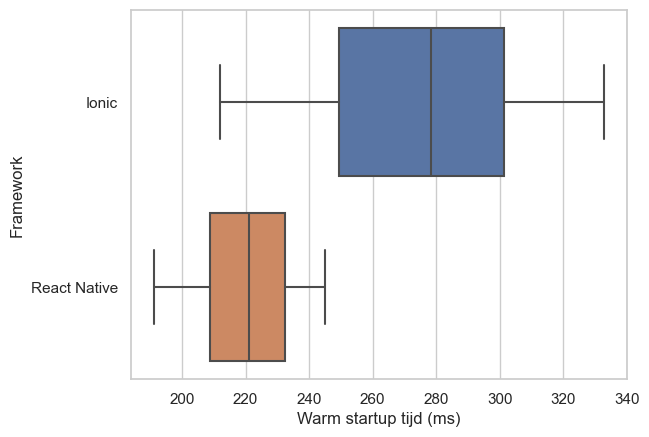
\includegraphics[width=0.7\linewidth]{img/boxplotWarm}
  \caption{Boxplot van de warm startup-tijd voor Ionic en React Native applicaties}
  \label{fig:Boxplot van de warm startup-tijd voor Ionic en React Native applicaties}
\end{figure}

Ook voor deze gegevens werd er een boxplot gemaakt (zie Figuur \ref{fig:Boxplot van de warm startup-tijd voor Ionic en React Native applicaties}). Vervolgens werd er opnieuw een t-test uitgevoerd om te zien of er een significant verschil is tussen de gemiddelden van de warm startup-tijden bij beide frameworks. De nulhypothese was dat er geen verschil is tussen de gemiddelden en als alternatieve hypothese dat de resultaten voor React Native lager zouden zijn dan die van Ionic. Deze test werd opnieuw uitgevoerd met een significantieniveau van \(0.05\). De p-waarde had als waarde \(8.244^{-8}\), wat lager is dan de significantieniveau. Hieruit kan geconcludeerd worden dat de nulhypothese kan verworpen worden en dat React Native over het algemeen iets sneller blijkt te zijn dan Ionic, alhoewel dit verschil slechts over enkele milliseconden gaat en eigenlijk op gebruikersniveau quasi niet veel voorstelt.


\subsection{Interactie}
\label{subsec:interactie}

De interactie met de applicaties werd als vrij responsief ervaren. Het was mogelijk om vrij snel te schakelen tussen de verschillende video's door op de knoppen te klikken. Vanaf een knop werd aangeklikt, reageerde de interface onmiddellijk door de videospeler te renderen en binnen een tijdspanne van 2-3 seconden de video af te spelen. Ondanks dat er een pauze was tussen het klikken op de knop en het effectief inladen van de video, werd deze pauze niet als storend ervaren en werd de video snel en vloeiend afgespeeld. Bij het meten werd er deze keer opnieuw gekeken naar de Android Profiler en de logs van Android Studio om de reactietijden te meten. De resultaten van deze metingen zijn te vinden in de tabel op de volgende pagina.

%erbij vermelden dat emulator stottert


\begin{table}[htbp]
  \centering
  \begin{tabular}{|c|c|c|}
  \hline
  \textbf{Testscenario} & \textbf{Ionic} & \textbf{React Native} \\
  \hline
  1 & 2s 807ms & 3s 56ms \\
  \hline
  2 & 2s 159ms & 2s 218ms \\
  \hline
  3 & 2s 123ms & 3s 177ms \\
  \hline
  4 & 2s 412ms & 2s 979ms \\
  \hline
  5 & 2s 788ms & 2s 762ms \\
  \hline
  6 & 2s 437ms & 2s 731ms \\
  \hline
  7 & 2s 354ms & 2s 964ms \\
  \hline
  8 & 2s 617ms & 2s 916ms \\
  \hline
  9 & 2s 622ms & 2s 775ms \\
  \hline
  10 & 2s 201ms & 2s 549ms \\
  \hline
  11 & 2s 193ms & 2s 636ms \\
  \hline
  12 & 2s 773ms & 2s 985ms \\
  \hline
  13 & 2s 111ms & 2s 909ms \\
  \hline
  14 & 2s 479ms & 3s 41ms \\
  \hline
  15 & 2s 671ms & 2s 963ms \\
  \hline
  16 & 2s 306ms & 2s 843ms \\
  \hline
  17 & 2s 828ms & 2s 872ms \\
  \hline
  18 & 2s 584ms & 2s 469ms \\
  \hline
  19 & 2s 453ms & 2s 760ms \\
  \hline
  20 & 2s 404ms & 2s 932ms \\
  \hline
  \textbf{Gemiddelde} & \textbf{2s 466ms} & \textbf{2s 827ms} \\
  \hline
  \end{tabular}
  \caption{Tijd voor het inladen van de video na het klikken op een knop voor Ionic en React Native applicaties}
  \label{tab:warm_startup}
\end{table}

\begin{figure}
  \centering
  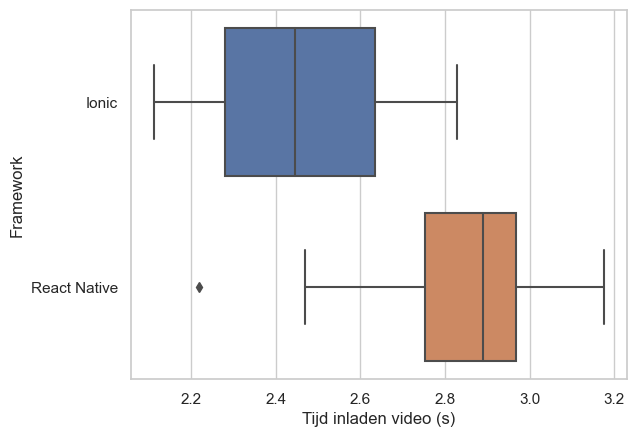
\includegraphics[width=0.7\linewidth]{img/boxplotInteraction}
  \caption{Boxplot van de tijd voor het inladen van de video na het klikken op een knop voor Ionic en React Native applicaties}
  \label{fig:Boxplot van de tijd voor het inladen van de video na het klikken op een knop voor Ionic en React Native applicaties}
\end{figure}

Indien voor dit testscenario opnieuw de t-test uitgevoerd wordt met een significantieniveau van \(0.05\), krijgt de p-waarde een waarde van \(8.624^{-6}\). Dit is opnieuw lager dan het significantieniveau en betekent dat ook hier Ionic een kleine voorsprong heeft op React Native. Op zich lijkt dit verschil misschien aanvankelijk niet zo groot, maar in een situatie waarbij de gebruiker snel wilt schakelen tussen verschillende video's, om bijvoorbeeld de juiste video te vinden, kan dit na enkele keren toch wel een merkbaar verschil beginnen worden tussen beide applicaties. Vanwege deze reden wordt Ionic hier als een betere keuze beschouwd op vlak van het ophalen en inladen van de video's.


\subsection{Video afspeelprestaties}
\label{subsec:video-afspeelprestaties}

Bij het afspelen van video's op zowel React als Ionic, werd over het algemeen een hoge afspeelkwaliteit ervaren. De video's werd telkens in hoge kwaliteit met een goed geluid afgespeeld. Echter werden er momenten waargenomen waarbij er enige haperingen optraden, vooral bij het afspelen van video's met de hogere resolutie van 4k. Hierdoor begon ook de geluidssynchronisatie het wat te begeven en leek het aanvankelijk alsof beide applicaties wel wat moeite bleken te hebben.

Echter op basis van onderstaande metingen, blijkt dat de haperingen eerder te wijten zijn aan de emulator dan aan de applicaties zelf. Dit wordt ondersteund door observaties van het CPU-gebruik die op geen enkel moment werd overbelast. Daarnaast hapert de emulator zelf ook bij het algemeen gebruik, zoals bij het scrollen tussen de geïnstalleerde applicaties, met andere woorden bij laag intensief gebruik.


\subsection{CPU-gebruik}
\label{subsec:cpu-gebruik}

Het CPU-gebruik werd telkens als volgt gemeten. Allereerst werd de applicatie de eerste keer opgestart nadat deze volledig was afgesloten. Vervolgens werd de eerste meting uitgevoerd totdat de applicatie volledig was opgestart. Aan de hand van de Android Profiler in Android Studio werd er gekeken naar het CPU-gebruik van de applicatie tijdens de opstartperiode en werd hiervan het gemiddelde genomen. De daaropvolgende test werd uitgevoerd nadat de app was opgestart, met andere woorden wanneer de app ``idle'' was. Dit gebeurde door opnieuw het gemiddelde van het CPU-gebruik te bepalen over een periode van exact 5 seconden. Hierna werden beide 1080p video's getest en als laatste de 4k video, waarbij de meting telkens begon vanaf het aanklikken van de knop tot exact 5 seconden later, wanneer de video al even aan het streamen was. Ook hiervan werd er telkens het gemiddelde genomen van het CPU-gebruik. Deze metingen werden een vijftiental keer herhaald om een beter beeld te verkrijgen van de variabiliteit van de data.

In de tabellen \ref{tab:cpu1} en \ref{tab:cpu2} zijn de resultaten van deze metingen te vinden. Hierbij werd de letter 'I' gebruikt voor Ionic en 'RN' voor React Native. Daarnaast verwijst de afkorting 'HD-1' naar de eerste 1080p video, 'HD-2' naar de tweede 1080p video en 'UHD' naar de 4k video.


\begin{table}[htbp]
  \centering
  \footnotesize
  \begin{tabular}{|c|c|c|c|c|}
      \hline
      \textbf{Testscenario} & \textbf{Startup I (\%)} & \textbf{Startup RN (\%)} & \textbf{Opgestart I (\%)} & \textbf{Opgestart RN (\%)} \\
      \hline
      1 & 30 & 21 & 0 & 1 \\
      \hline
      2 & 33 & 20 & 1 & 1 \\
      \hline
      3 & 29 & 22 & 1 & 0 \\
      \hline
      4 & 32 & 20 & 0 & 1 \\
      \hline
      5 & 30 & 18 & 0 & 0 \\
      \hline
      6 & 32 & 20 & 0 & 0 \\
      \hline
      7 & 28 & 19 & 1 & 1 \\
      \hline
      8 & 34 & 20 & 0 & 0 \\
      \hline
      9 & 26 & 21 & 1 & 1 \\
      \hline
      10 & 30 & 20 & 0 & 1 \\
      \hline
      11 & 28 & 21 & 0 & 1 \\
      \hline
      12 & 33 & 19 & 1 & 1 \\
      \hline
      13 & 30 & 20 & 1 & 0 \\
      \hline
      14 & 32 & 20 & 0 & 1 \\
      \hline
      15 & 28 & 19 & 1 & 0 \\
      \hline
      \textbf{Gemiddelde} & \textbf{30.3} & \textbf{20} & \textbf{0.47} & \textbf{0.60} \\
      \hline
  \end{tabular}
  \caption{CPU-gebruik van de Ionic en React Native applicaties bij het opstarten (Startup) en wanneer de applicatie opgestart is (Opgestart). Hierbij verwijst de letter 'I' naar Ionic en 'RN' naar React Native.}
  \label{tab:cpu1}
\end{table}

\begin{table}[htbp]
  \centering
  \footnotesize
  \begin{tabular}{|c|c|c|c|c|c|c|}
      \hline
      \textbf{Testscenario} & \textbf{HD-1 I (\%)} & \textbf{HD-1 RN (\%)} & \textbf{HD-2 I (\%)} & \textbf{HD-2 RN (\%)} & \textbf{UHD I (\%)} & \textbf{UHD RN (\%)} \\
      \hline
      1 & 20 & 32 & 22 & 40 & 51 & 56 \\
      \hline
      2 & 18 & 31 & 24 & 44 & 38 & 63 \\
      \hline
      3 & 26 & 35 & 19 & 34 & 42 & 61 \\
      \hline
      4 & 21 & 29 & 23 & 29 & 59 & 70 \\
      \hline
      5 & 21 & 33 & 25 & 36 & 39 & 65 \\
      \hline
      6 & 19 & 30 & 25 & 28 & 56 & 60 \\
      \hline
      7 & 23 & 36 & 22 & 31 & 34 & 50 \\
      \hline
      8 & 16 & 34 & 26 & 38 & 48 & 71 \\
      \hline
      9 & 24 & 28 & 23 & 45 & 46 & 62 \\
      \hline
      10 & 19 & 29 & 20 & 33 & 52 & 69 \\
      \hline
      11 & 20 & 30 & 24 & 40 & 57 & 75 \\
      \hline
      12 & 16 & 31 & 21 & 38 & 38 & 73 \\
      \hline
      13 & 22 & 33 & 25 & 27 & 55 & 57 \\
      \hline
      14 & 18 & 32 & 24 & 34 & 43 & 66 \\
      \hline
      15 & 23 & 30 & 19 & 41 & 50 & 52 \\
      \hline
      \textbf{Gemiddelde} & \textbf{20.4} & \textbf{31.5} & \textbf{22.8} & \textbf{35.9} & \textbf{47.2} & \textbf{63.3} \\
      \hline
  \end{tabular}
  \caption{CPU-gebruik van de Ionic en React Native applicaties bij het afspelen van video's. De letter 'I' verwijst naar Ionic en 'RN' naar React Native respectievelijk.}
  \label{tab:cpu2}
\end{table}

\begin{table}[htbp]
  \centering
  \footnotesize
  \begin{tabular}{|c|c|c|}
      \hline
      \textbf{Testvideo} & \textbf{P-waarde} & \textbf{Beste resultaat} \\
      \hline
      Eerste HD-video & \(2.574^{-12}\) & Ionic \\
      \hline
      Tweede HD-video & \(5.975^{-8}\) & Ionic \\
      \hline
      UHD-video & \(1.958^{-6}\) & Ionic \\
      \hline
  \end{tabular}
  \caption{Resultaten van de t-test voor het CPU-gebruik bij het afspelen van video's}
  \label{tab:cpu_ttest}
\end{table}

\begin{figure}
  \centering
  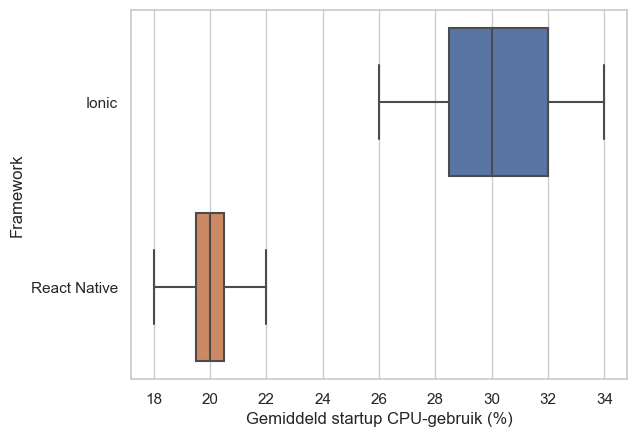
\includegraphics[width=0.7\linewidth]{img/cpu/startup}
  \caption{Boxplot van het CPU-gebruik van de Ionic en React Native applicaties bij het opstarten}
  \label{fig:Boxplot van het CPU-gebruik van de Ionic en React Native applicaties bij het opstarten}
\end{figure}

\begin{figure}
  \centering
  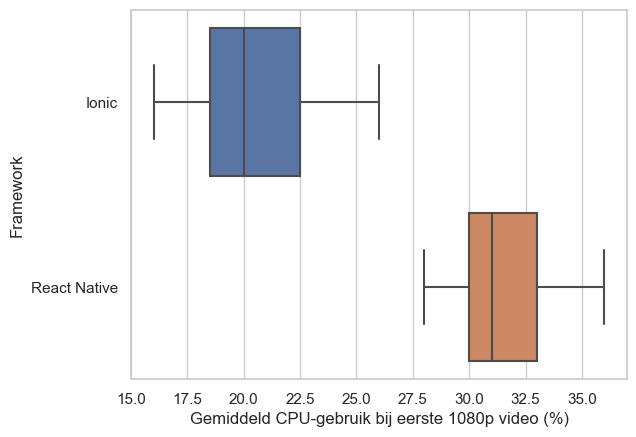
\includegraphics[width=0.7\linewidth]{img/cpu/HD1}
  \caption{Boxplot van het CPU-gebruik van de Ionic en React Native applicaties bij het afspelen van de eerste 1080p video}
  \label{fig:Boxplot van het CPU-gebruik van de Ionic en React Native applicaties bij het afspelen van de eerste 1080p video}
\end{figure}

\begin{figure}
  \centering
  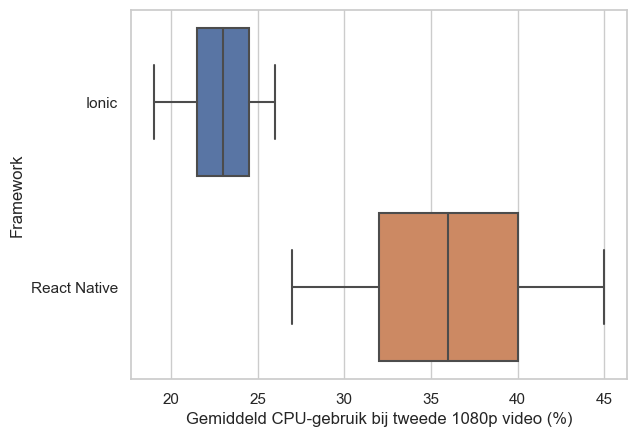
\includegraphics[width=0.7\linewidth]{img/cpu/HD2}
  \caption{Boxplot van het CPU-gebruik van de Ionic en React Native applicaties bij het afspelen van de tweede 1080p video}
  \label{fig:Boxplot van het CPU-gebruik van de Ionic en React Native applicaties bij het afspelen van de tweede 1080p video}
\end{figure}

\begin{figure}
  \centering
  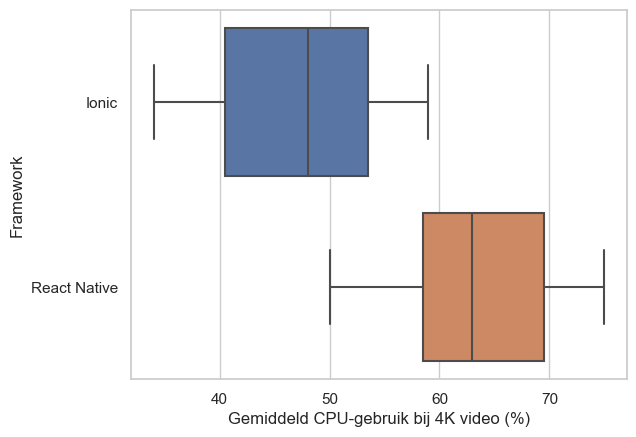
\includegraphics[width=0.7\linewidth]{img/cpu/4k}
  \caption{Boxplot van het CPU-gebruik van de Ionic en React Native applicaties bij het afspelen van de 4k video}
  \label{fig:Boxplot van het CPU-gebruik van de Ionic en React Native applicaties bij het afspelen van de 4k video}
\end{figure}


Bij het opstarten van de applicatie vertoonde de Ionic-applicatie een hoger gemiddeld CPU-gebruik in tegenstelling tot React Native. Dit is te zien in de bovenstaande tabel en de bijhorende boxplot op Figuur \ref{fig:Boxplot van het CPU-gebruik van de Ionic en React Native applicaties bij het opstarten}. Echter toen beide applicaties waren opgestart, bleef het CPU-gebruik van beide applicaties ongeveer op hetzelfde niveau hangen, namelijk rond de 0 en 1 procent. Aangezien het hier slechts over een zeer laag percentage gaat en eigenlijk bijna verwaarloosbaar is, werd hier niet dieper op ingegaan. Er kan namelijk moeilijk over een significant performantieverschil gesproken worden wanneer het CPU-gebruik zo laag is.


Voor de resultaten bij het afspelen van de video's waren er toch wat verschillen op te merken. Op basis van de grafieken en tabellen bleek Ionic hier steeds de overduidelijke winnaar te zijn. Maar om dit toch statistisch te onderbouwen, werd er telkens een t-test uitgevoerd met als significantieniveau opnieuw \(0.05\). De resultaten hiervan zijn te vinden in de tabel \ref{tab:cpu_ttest}. Hieruit blijkt dat er een significant verschil is tussen het CPU-gebruik van Ionic en React Native bij het afspelen van video's. Uit de tabel \ref{tab:cpu2} kan er bovendien zelf een verband worden gelegd tussen de resolutie van de video en het CPU-gebruik. Zo is het CPU-gebruik bij het afspelen van een 4k video aanzienlijk hoger dan bij een 1080p video. Dit heeft dan weer te maken met het feit dat een hogere resolutie meer dataverwerking vereist en dus ook meer CPU-gebruik met zich meebrengt.


\subsection{Geheugengebruik}
\label{subsec:geheugengebruik}

Het geheugengebruik werd ook gemeten aan de hand van de Android Profiler in Android Studio. Hierbij werd er gekeken naar het piek-geheugengebruik na het opstarten van de applicatie en bij het afspelen van de video's. De metingen werden telkens vastgelegd in megabytes (MB) en werden een vijftiental keer herhaald. De reden om de piek-geheugengebruik te meten, was omdat het RAM-geheugen na een bepaalde activiteit zoals het inladen van een video, begon af te vlakken tot een vast punt. Dit punt werd dan als piek-geheugengebruik beschouwd. De resultaten van deze metingen zijn te vinden in de tabellen \ref{tab:memory1} en \ref{tab:memory2}. Bij deze tweede tabel is er opnieuw sprake van de afkortingen 'I' en 'RN' voor respectievelijk Ionic en React Native. Daarnaast verwijst 'HD-1' nog steeds naar de eerste 1080p video, 'HD-2' naar de tweede 1080p video en 'UHD' naar de 4k video.

Op basis van de resultaten bleek ook hier dat Ionic een grote voorsprong had op React Native. Enkel na de initiële opstart van de applicatie was er slechts een klein verschil op te merken tussen beide frameworks. Hoe hoger de resolutie van de video, hoe meer RAM-geheugen in gebruik werd genomen door React Native, terwijl Ionic relatief stabiel rond dezelfde waarden bleef hangen. In tabel \ref{tab:memory_ttest} zijn de resultaten van de t-test te vinden met een significantieniveau van \(0.05\). Hieruit kan vastgesteld worden dat Ionic de beste keuze blijkt te zijn op vlak van geheugengebruik bij het streamen.

\begin{table}[htbp]
  \centering
  \footnotesize
  \begin{tabular}{|c|c|c|}
      \hline
      \textbf{Scenario} & \textbf{P-waarde} & \textbf{Beste resultaat} \\
      \hline
      Na opstarten & \(0.00046\) & Ionic \\
      \hline
      Eerste HD-video & \(1.371^{-11}\) & Ionic \\
      \hline
      Tweede HD-video & \(1.807^{-10}\) & Ionic \\
      \hline
      UHD-video & \(7.690^{-25}\) & Ionic \\
      \hline
  \end{tabular}
  \caption{Resultaten van de t-test voor het CPU-gebruik bij het afspelen van video's}
  \label{tab:memory_ttest}
\end{table}

\begin{table}[htbp]
  \centering
  \begin{tabular}{|c|c|c|}
      \hline
      \textbf{Testscenario} & \textbf{Opgestart I (MB)} & \textbf{Opgestart RN (MB)} \\
      \hline
      1 & 113.2 & 113.5 \\
      \hline
      2 & 114.6 & 117.2 \\
      \hline
      3 & 115.5 & 115.1 \\
      \hline
      4 & 113.8 & 118.0 \\
      \hline
      5 & 112.4 & 114.3 \\
      \hline
      6 & 112.7 & 119.1 \\
      \hline
      7 & 114.9 & 113.8 \\
      \hline
      8 & 112.8 & 117.5 \\
      \hline
      9 & 115.9 & 116.7 \\
      \hline
      10 & 113.6 & 114.9 \\
      \hline
      11 & 114.1 & 115.3 \\
      \hline
      12 & 113.1 & 117.8 \\
      \hline
      13 & 115.2 & 113.4 \\
      \hline
      14 & 114.3 & 116.1 \\
      \hline
      15 & 112.5 & 118.6 \\
      \hline
      \textbf{Gemiddelde} & \textbf{113.9} & \textbf{116.1} \\
      \hline
  \end{tabular}
  \caption{Piek-geheugengebruik van Ionic en React Native applicaties wanneer de applicatie opgestart is. Hierbij verwijst de letter 'I' naar Ionic en 'RN' naar React Native.}
  \label{tab:memory1}
\end{table}

\begin{table}[htbp]
  \centering
  \footnotesize
  \scalebox{0.9}{
    \begin{tabular}{|c|c|c|c|c|c|c|}
        \hline
        \textbf{Testscenario} & \textbf{HD-1 I (MB)} & \textbf{HD-1 RN (MB)} & \textbf{HD-2 I (MB)} & \textbf{HD-2 RN (MB)} & \textbf{UHD I (MB)} & \textbf{UHD RN (MB)} \\
        \hline
        1 & 121.7 & 136.7 & 120.5 & 133.2 & 122.5 & 149.5 \\
        \hline
        2 & 118.9 & 141.0 & 119.3 & 140.3 & 122.9 & 153.0 \\
        \hline
        3 & 120.2 & 139.8 & 118.7 & 145.7 & 119.9 & 152.4 \\
        \hline
        4 & 121.5 & 137.5 & 118.5 & 142.9 & 121.2 & 151.1 \\
        \hline
        5 & 117.5 & 135.9 & 120.7 & 132.1 & 121.6 & 150.6 \\
        \hline
        6 & 118.3 & 143.2 & 118.4 & 138.5 & 118.8 & 155.2 \\
        \hline
        7 & 121.8 & 148.6 & 117.9 & 145.2 & 121.8 & 154.1 \\
        \hline
        8 & 121.4 & 151.3 & 118.3 & 149.5 & 121.3 & 156.0 \\
        \hline
        9 & 120.1 & 142.1 & 121.5 & 138.7 & 118.6 & 152.7 \\
        \hline
        10 & 119.7 & 137.4 & 118.4 & 136.2 & 121.5 & 150.8 \\
        \hline
        11 & 117.2 & 140.6 & 120.9 & 144.9 & 121.0 & 153.6 \\
        \hline
        12 & 122.2 & 147.2 & 121.2 & 148.3 & 120.9 & 155.7 \\
        \hline
        13 & 118.2 & 135.8 & 120.3 & 133.7 & 121.4 & 149.9 \\
        \hline
        14 & 121.9 & 149.0 & 120.1 & 146.6 & 119.8 & 154.5 \\
        \hline
        15 & 117.4 & 150.1 & 121.0 & 147.5 & 120.3 & 151.3 \\
        \hline
        \textbf{Gemiddelde} & \textbf{119.9} & \textbf{142.4} & \textbf{119.7} & \textbf{141.6} & \textbf{120.9} & \textbf{152.7} \\
        \hline
    \end{tabular}
  }
  \caption{Geheugengebruik voor Ionic en React Native applicaties bij het afspelen van video's. De letter 'I' verwijst naar Ionic en 'RN' naar React Native respectievelijk.}
  \label{tab:memory2}
\end{table}

\begin{figure}
  \centering
  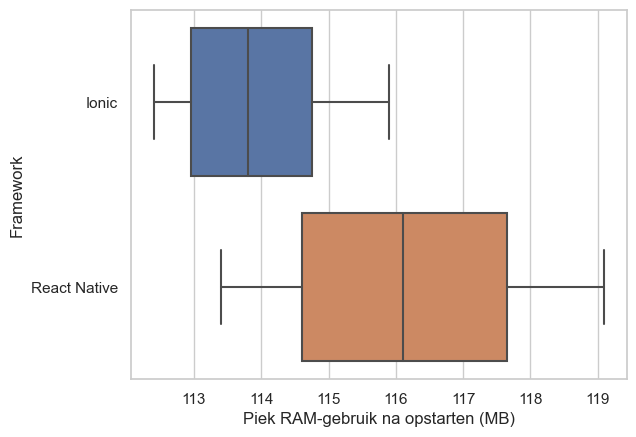
\includegraphics[width=0.7\linewidth]{img/ram/loaded}
  \caption{Boxplot van het piek-geheugengebruik van Ionic en React Native applicaties wanneer de applicatie opgestart is}	
  \label{fig:Boxplot van het piek-geheugengebruik van Ionic en React Native applicaties wanneer de applicatie opgestart is}
\end{figure}

\begin{figure}
  \centering
  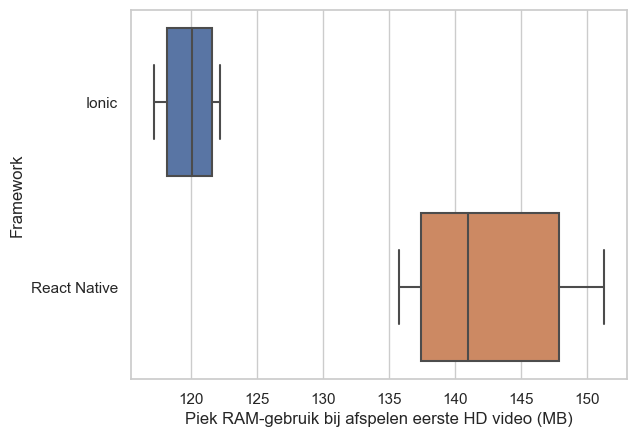
\includegraphics[width=0.7\linewidth]{img/ram/HD1}
  \caption{Boxplot van het piek-geheugengebruik van Ionic en React Native applicaties bij het afspelen van de eerste 1080p video}
  \label{fig:Boxplot van het piek-geheugengebruik van Ionic en React Native applicaties bij het afspelen van de eerste 1080p video}
\end{figure}

\begin{figure}
  \centering
  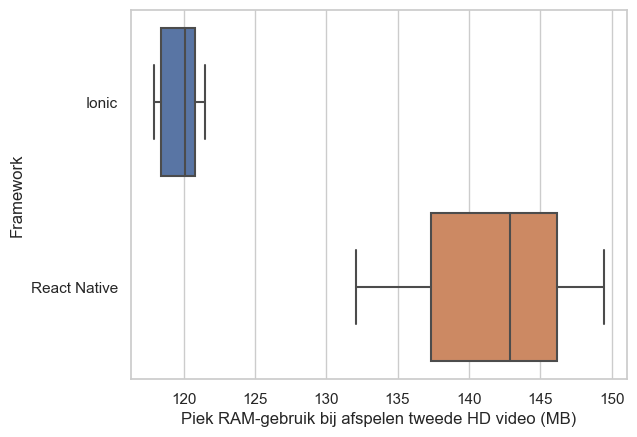
\includegraphics[width=0.7\linewidth]{img/ram/HD2}
  \caption{Boxplot van het piek-geheugengebruik van Ionic en React Native applicaties bij het afspelen van de tweede 1080p video}
  \label{fig:Boxplot van het piek-geheugengebruik van Ionic en React Native applicaties bij het afspelen van de tweede 1080p video}
\end{figure}

\begin{figure}
  \centering
  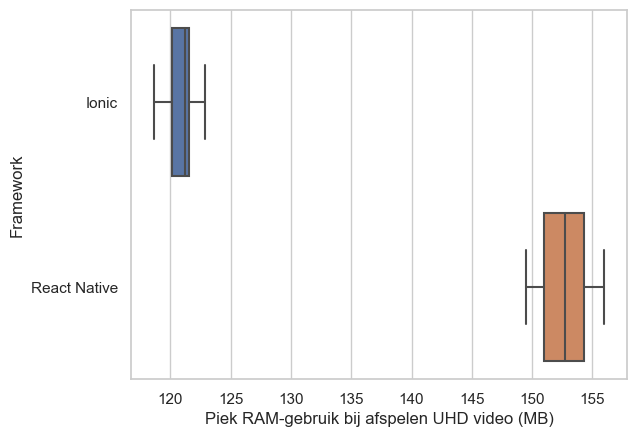
\includegraphics[width=0.7\linewidth]{img/ram/4k}
  \caption{Boxplot van het piek-geheugengebruik van Ionic en React Native applicaties bij het afspelen van de 4k video}
  \label{fig:Boxplot van het piek-geheugengebruik van Ionic en React Native applicaties bij het afspelen van de 4k video}
\end{figure}


\subsection{Groottes van de applicaties}
\label{subsec:groottes-van-de-applicaties}

In dit laatste onderdeel zal er nog even kort stilgestaan worden bij de groottes van de APK-bestanden. Dit heeft niet noodzakelijk een impact op de performantie, maar toont wel een interessante vergelijking aan hoe hun interne structuur en de manier waarop ze gebouwd zijn, invloed kunnen hebben op de bestandsgrootte. De APK-bestandsgrootte werd gemeten aan de hand van de grootte van de APK-bestanden die gegenereerd werden bij het bouwen van de applicaties. Het APK-bestand van React Native telde 155 MB, terwijl die van Ionic een gigantisch stuk kleiner was met slechts 3,76 MB. Dit valt te wijten aan het gebruik van native componenten bij React Native. Bij React Native is er meer data vereist om te weten welke componenten er allemaal moeten gebruikt worden en hoe deze moeten samenwerken. Ionic daarentegen maakt gebruik van enkel de webview-engine van het toestel (in dit geval), waardoor de componenten niet in de app zelf moeten ingeladen worden. De webtechnologieën zoals HTML en CSS worden namelijk gebruikt om de componenten te renderen, wat uiteindelijk resulteert in een lichtere en efficiëntere APK-bestandsgrootte.